\section{Aufbau und Durchführung}
\label{sec:Durchführung}
\subsection{Versuchsaufbau}
Kernstück des Aufbaus ist eine transparente Plexiglas Grundplatte. Auf dieser befinden sich ein grüner Laser der Wellenlänge $\lambda = \SI{532}{nm}$ und ein roter Laser
der Wellenlänge $\lambda = \SI{635}{nm}$. Die Laser sind übereinander verbaut und lassen sich in einem Halbkreis bewegen. In der Mitte des Halbkreises lassen sich verschiedene
optische Elemente einbauen. Zum Schutz vor dem Laser-Licht ist am Ende des Halbkreises ein Reflexionsschirm angebracht. Für die Durchführung und Messungen werden die benötigten
optischen Elemente mit Halterungen befestigt und die Versuchsvorlagen zur Messung des Winkels unter die Platte gelegt. In \autoref{fig:aufbau} ist ein Foto des Versuchaufbaus
und in \autoref{fig:elemente} ein Foto der optischen Elemente und Halterungen abgebildet.
\begin{figure}[H]
    \centering
    \begin{subfigure}[b]{0.49\textwidth}
        \centering
        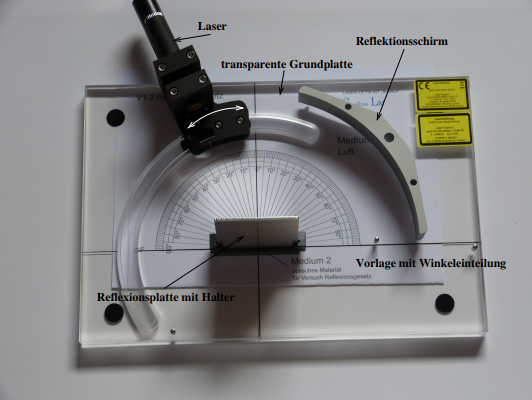
\includegraphics[width=6cm, height=5cm]{img/durchfuehrung1.png}
        \caption[]
        {{\small Versuchsaufbau \cite{V400}.}}    
        \label{fig:aufbau}
    \end{subfigure}
    \hfill
    \begin{subfigure}[b]{0.49\textwidth}  
        \centering 
        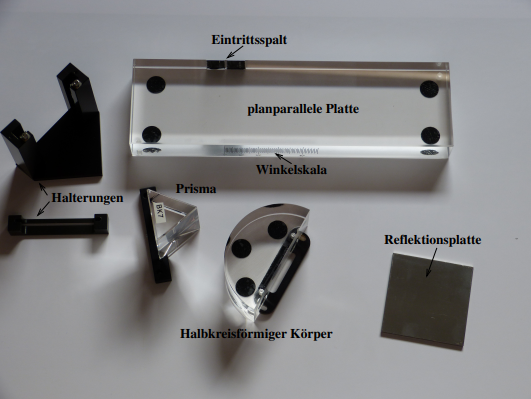
\includegraphics[width=6cm, height=5cm]{img/durchfuehrung2.png}
        \caption[]
        {{\small Optische Elemente \cite{V400}.}}    
        \label{fig:elemente}
    \end{subfigure}
\end{figure}
Beim Aufbauen der Teil-Experimente ist es wichtig, die Elemente nur am Rand oder den Halterungen anzufassen, damit diese nicht beschädigt werden.
\subsection{Durchführung}
\textbf{Erste Aufgabe:}\\
Für diesen Teil wird der grüne Laser, die Vorlage A und der Halter mit dem Spiegel verwendet. Das Reflexionsgesetz soll überprüft werden, d.h. es werden
7 Einfalls- und der zugehörige Reflexionswinkel aufgenommen.\\
\textbf{Zweite Aufgabe:}\\
In diesem Teil werden wieder der grüne Laser und die Vorlage A verwendet. Mit der planparallelen Platte soll das Brechungsgesetz überprüft werden.
Es werden wieder 7 Einfalls und der zugehörige Brechungswinkel aufgenommen.\\
\textbf{Dritte Aufgabe:}\\
Für diesen Teil können die Messwerte aus der vorherigen Aufgabe genutzt werden.\\
\textbf{Vierte Aufgabe:}\\
Anstelle der planparallelen Platte wird nun ein Prisma eingebaut. Die Vorlage A wird durch die Vorlage C ersetzt. Da sowohl der grüne als auch der rote Laser
verwendet werden sollen, muss der Reflexionsschutz erhöht werden. Es soll für 5 verschiedene Einfallswinkel, die Ausfallswinkel aus dem Prisma gemessen werden.\\
\textbf{Fünfte Aufgabe:}\\
In diesem Teil soll die Beugung am Gitter untersucht werden. Der Laser soll so justiert werden, dass das Laser-Licht die Winkelskala des Transmissionsschirmes
bei 0° trifft. Dadurch sind die Ablenkwinkel direkt ablesbar. Ein Beugungsgitter mit einer Gitterkonstanten $d = \SI{600}{\frac{1}{mm}}$ wird eingesetzt. 
Gemessen werden sollen die Beugungsmaxima des roten und grünen Lasers.
\newpage